\chapter{New Revolutions in Particle Physics: Basic Concepts}

These notes follow Lecture 1 of Leonard Susskind's \emph{Particle Physics 1: Basic Concepts}. The story is told, as in the lecture, for logical force rather than strict chronology, and the curation of the lecture materials is due to LazyingArt LLC. The opening question is ancient and still governs the subject: is nature discrete, or is it continuous? From that question we are led, step by step, through chemistry, radioactivity, light as a classical wave, light as a quantum, relativity, natural units, and finally to the practical rule that drives particle physics: to see smaller things we need shorter wavelengths, and shorter wavelengths require larger momentum and energy.

\section{Discreteness, Continuity, and the First Chemical Evidence}

Particle physics is introduced here in the broadest possible way. We do not begin with a catalogue of particles. We begin with two rival pictures of matter.

The first picture says that matter comes in indivisible units. The ancient word was \emph{atom}; in the lecture Susskind immediately relaxes the language and says: let us just call such discrete units particles. The second picture says the opposite: matter is not built from localized lumps at all, but is continuously distributed, smeared out through space. In that language one speaks of fields, and the lecture is careful to say what a field is: a function on space. A density is a field. The electric field is a field. The magnetic field is a field. A field is not a little object sitting somewhere; it is something defined throughout a region of space.

Already at the beginning we are warned not to expect a simple victory for one side. Quantum mechanics will eventually force us to say that the particle picture and the continuum picture are both right and both incomplete. But before that subtlety appears, we want evidence.

The first serious evidence for discreteness enters through chemistry. Dalton noticed that the mass of a fixed number of molecules of a substance comes, to good approximation, in integer multiples of the mass of the same number of hydrogen molecules. The point is not exact arithmetic perfection. The point is that the ratios are near integers. Not three halves, not \(\pi\), but integers. That is just the sort of pattern one expects if matter is being built from some underlying units.

From the modern point of view we can see what Dalton was really glimpsing. Ordinary matter is made from atoms, and the mass of an atom is concentrated overwhelmingly in protons and neutrons. Electrons are very light by comparison and contribute only a small correction. Protons and neutrons have nearly equal mass, and the nucleus of hydrogen contains just one proton. Therefore the mass of ordinary matter is, to first approximation, counted in units of proton-or-neutron mass, and Dalton's integral pattern becomes intelligible. The lecture does not overstate this: it is an approximation, not an exact law, but it is a very revealing approximation.

By the end of nineteenth-century chemistry the elements themselves looked like the elementary building blocks. There were roughly a hundred kinds of atoms, and it was natural to think that the story stopped there. Then, as the lecture puts it, all hell broke loose.

\section{Radioactivity and the First Particle Beam}

The next step is radioactivity, and the lecture treats it as the first real particle-physics experiment. The story begins with a happy accident. A radioactive source affects a photographic plate as if some invisible radiation had struck it. Becquerel then tries to study that radiation more carefully. He buries the source in a block of lead, drills a narrow hole through the lead, and places a photographic plate some distance away. The hole collimates the emission, and what had been a vague effect becomes a narrow beam.

\begin{figure}[h]
\centering
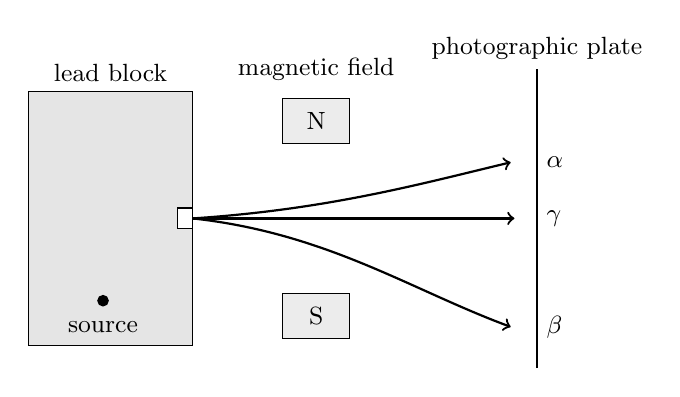
\begin{tikzpicture}[scale=0.95]
\draw[fill=gray!20] (0,-1.7) rectangle (2.2,1.7);
\draw[fill=white] (2.0,-0.14) rectangle (2.2,0.14);
\draw[fill=black] (1.0,-1.1) circle (0.07);
\node at (1.0,-1.45) {\small source};

\draw[thick] (6.8,-2.0) -- (6.8,2.0);
\node[above] at (6.8,2.0) {\small photographic plate};

\draw[fill=gray!15] (3.4,1.0) rectangle (4.3,1.6);
\draw[fill=gray!15] (3.4,-1.6) rectangle (4.3,-1.0);
\node at (3.85,1.3) {\small N};
\node at (3.85,-1.3) {\small S};

\draw[thick,->] (2.2,0.0) -- (6.5,0.0);
\draw[thick,->] (2.2,0.0) .. controls (4.0,0.12) and (5.2,0.45) .. (6.45,0.75);
\draw[thick,->] (2.2,0.0) .. controls (4.0,-0.2) and (5.1,-0.95) .. (6.45,-1.45);

\node[right] at (6.8,0.75) {\small \(\alpha\)};
\node[right] at (6.8,0.0) {\small \(\gamma\)};
\node[right] at (6.8,-1.45) {\small \(\beta\)};

\node at (1.1,1.95) {\small lead block};
\node at (3.85,2.0) {\small magnetic field};
\end{tikzpicture}
\caption{A schematic version of Becquerel's collimated radioactive source. In the lecture this becomes the first particle beam, and a magnetic field separates the radiation into \(\alpha\), \(\beta\), and \(\gamma\) components.}
\end{figure}

That is already a striking development: something is being emitted in a directed beam. Then a magnetic field is brought near the beam, and the beam separates into three branches. One branch goes straight through, as if the magnetic field were absent. The other two bend in opposite directions, as charged objects should in a magnetic field, and they do not bend equally strongly.

From the modern point of view the identifications are
\begin{equation}
\begin{aligned}
\beta\text{-radiation}&=\text{electrons},\\
\alpha\text{-radiation}&=\text{helium nuclei},\\
\gamma\text{-radiation}&=\text{photons}.
\end{aligned}
\end{equation}
But the lecture does not move too quickly. It pauses over what was actually learned. Whatever was coming out of the source behaved as if it came in distinguishable components, and if the source were dilute enough one could imagine the screen registering arrivals one at a time: blip, blip, blip. Alpha arrives in little bundles. Beta arrives in little bundles. Gamma too.

At this stage \(\gamma\)-radiation is the real mystery. It is neutral, it reaches the screen one event at a time, and yet there is no familiar neutral particle available to explain it. The lecture uses exactly that unresolved tension to pivot into the next subject. Gamma, it turns out, is light. But once gamma is recognized as light, a deeper problem appears, because light already seemed to belong to the opposite camp.

\section{Light as a Classical Wave}

Gamma radiation is announced to be light, or rather very high-energy light. But that statement does not immediately settle anything. It sharpens the problem. For light was the strong classical example of something continuous, something field-like, something that looked very much not like a particle.

The lecture first secures the classical case before permitting any quantum rescue. Suppose electromagnetic radiation is emitted from a source. The source might be a macroscopic antenna; it might equally well be an atom, which in this context acts as a perfectly good microscopic antenna. If light were merely a spray of bullets, then a small hole in an obstruction should produce a small sharp spot on a screen. Instead one gets a fuzzier region. That is suggestive, but not decisive. One might still imagine particles being deflected by the edges of the opening.

The decisive experiment uses two openings rather than one. If light were only particles, then two holes would simply give two smeared spots superimposed on one another. But that is not what happens. One sees alternating bright and dark bands. The bright bands come from constructive interference, where wave crests meet wave crests. The dark bands come from destructive interference, where a crest from one opening meets a trough from the other.

\begin{figure}[h]
\centering
\resizebox{\linewidth}{!}{%
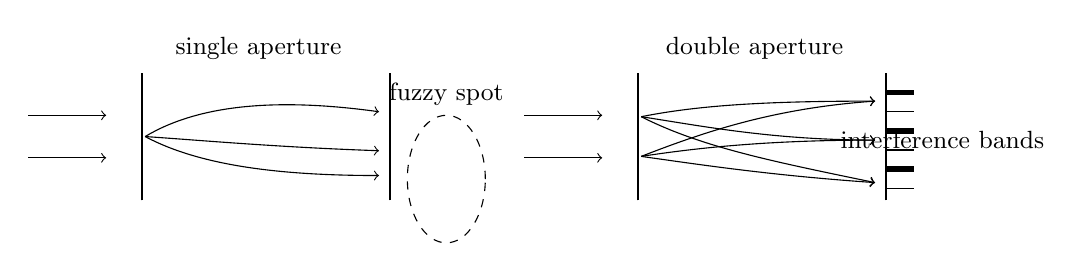
\begin{tikzpicture}[scale=0.9]
\draw[->] (-0.3,1.4) -- (0.8,1.4);
\draw[->] (-0.3,0.8) -- (0.8,0.8);
\draw[thick] (1.3,0.2) -- (1.3,2.0);
\draw[thick,white,line width=5pt] (1.3,1.0) -- (1.3,1.2);
\draw[thick] (1.3,0.2) -- (1.3,2.0);
\draw[thick] (4.8,0.2) -- (4.8,2.0);
\draw[->] (1.35,1.1) .. controls (2.1,1.55) and (3.2,1.65) .. (4.65,1.45);
\draw[->] (1.35,1.1) .. controls (2.1,1.05) and (3.2,0.95) .. (4.65,0.9);
\draw[->] (1.35,1.1) .. controls (2.1,0.7) and (3.2,0.55) .. (4.65,0.55);
\draw[dashed] (5.6,0.5) ellipse (0.55 and 0.9);
\node at (2.95,2.35) {\small single aperture};
\node at (5.6,1.7) {\small fuzzy spot};

\draw[->] (6.7,1.4) -- (7.8,1.4);
\draw[->] (6.7,0.8) -- (7.8,0.8);
\draw[thick] (8.3,0.2) -- (8.3,2.0);
\draw[thick,white,line width=5pt] (8.3,0.75) -- (8.3,0.9);
\draw[thick,white,line width=5pt] (8.3,1.3) -- (8.3,1.45);
\draw[thick] (8.3,0.2) -- (8.3,2.0);
\draw[thick] (11.8,0.2) -- (11.8,2.0);

\draw[->] (8.35,0.82) .. controls (9.2,1.15) and (10.2,1.5) .. (11.65,1.6);
\draw[->] (8.35,0.82) .. controls (9.2,0.95) and (10.2,1.05) .. (11.65,1.05);
\draw[->] (8.35,0.82) .. controls (9.2,0.7) and (10.2,0.55) .. (11.65,0.45);

\draw[->] (8.35,1.38) .. controls (9.2,1.55) and (10.2,1.6) .. (11.65,1.6);
\draw[->] (8.35,1.38) .. controls (9.2,1.25) and (10.2,1.05) .. (11.65,1.05);
\draw[->] (8.35,1.38) .. controls (9.2,0.95) and (10.2,0.75) .. (11.65,0.45);

\draw[line width=2pt] (11.8,1.72) -- (12.2,1.72);
\draw[line width=0.4pt] (11.8,1.45) -- (12.2,1.45);
\draw[line width=2pt] (11.8,1.18) -- (12.2,1.18);
\draw[line width=0.4pt] (11.8,0.91) -- (12.2,0.91);
\draw[line width=2pt] (11.8,0.64) -- (12.2,0.64);
\draw[line width=0.4pt] (11.8,0.37) -- (12.2,0.37);

\node at (9.95,2.35) {\small double aperture};
\node at (12.6,1.05) {\small interference bands};
\end{tikzpicture}
}%
\caption{Single-aperture spreading and double-aperture interference. In the lecture the first effect is suggestive, while the second really nails the wave character of light.}
\end{figure}

That is the experiment that really nails the wave theory. Maxwell then tells us what kind of wave light is. It is a wave of electric and magnetic field. If the wave propagates along some axis, the electric field oscillates transversely, the magnetic field oscillates transversely as well, and the two are perpendicular to one another.

\begin{figure}[h]
\centering
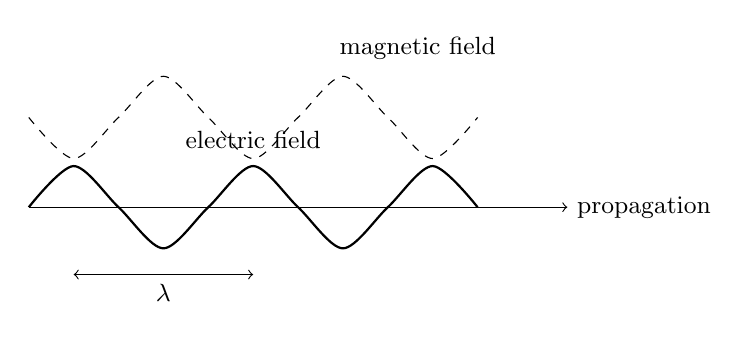
\begin{tikzpicture}[scale=0.95]
\draw[->] (0,0) -- (7.2,0);
\node[right] at (7.2,0) {\small propagation};

\draw[smooth,thick] plot coordinates {(0,0) (0.6,0.55) (1.2,0.0) (1.8,-0.55) (2.4,0.0) (3.0,0.55) (3.6,0.0) (4.2,-0.55) (4.8,0.0) (5.4,0.55) (6.0,0.0)};
\node[above] at (3.0,0.65) {\small electric field};

\draw[smooth,dashed] plot coordinates {(0,1.2) (0.6,0.65) (1.2,1.2) (1.8,1.75) (2.4,1.2) (3.0,0.65) (3.6,1.2) (4.2,1.75) (4.8,1.2) (5.4,0.65) (6.0,1.2)};
\node[above] at (5.2,1.85) {\small magnetic field};

\draw[<->] (0.6,-0.9) -- (3.0,-0.9);
\node[below] at (1.8,-0.9) {\small \(\lambda\)};
\end{tikzpicture}
\caption{A schematic electromagnetic wave. The lecture first secures light as a classical wave of electric and magnetic field before allowing the quantum puzzle to appear.}
\end{figure}

Once that classical picture is secure, the lecture pauses and deliberately slows down. Now we introduce notation. This is not a digression. It is preparation. The next equations will matter because photons will inherit them.

\section{Wave Kinematics}

The first quantity introduced is the wavelength. It is simply the spatial length of one full cycle of the wave. The board evidence for that moment is worth keeping, because the lecture begins a fresh little derivation there.

\begin{figure}[h]
\centering

\includegraphics[width=0.72\textwidth]{lecture_01_figure_02.png}
\caption{Introducing \(\lambda\) as wavelength. The board writing is only partially visible, but the transcript makes the intended notation clear.}
\end{figure}

So we write
\begin{equation}
\lambda = \text{wavelength}.
\end{equation}

Next comes the temporal description. If we stand still and let the wave pass us, the time required for one full oscillation is the period, which we denote by \(T\). In one period the wave advances by one wavelength. Therefore its speed is distance divided by time:
\begin{equation}
v=\frac{\lambda}{T}.
\end{equation}
For light the speed is \(c\), so
\begin{equation}
c=\frac{\lambda}{T}.
\end{equation}

It is then convenient to replace the period by its inverse, the frequency:
\begin{equation}
f=\frac{1}{T}.
\end{equation}
Substituting this into the previous equation gives the relation written on the board,
\begin{equation}
\lambda f = c.
\end{equation}

\begin{figure}[h]
\centering

\includegraphics[width=0.68\textwidth]{lecture_01_figure_03.png}
\caption{Frequency and wavelength relations on the board. The lecture has now moved from period to frequency and then to the light-wave relation \(\lambda f=c\).}
\end{figure}

That still uses cycles per second. The lecture now shifts to the notation physicists prefer. Instead of counting full turns per second, we count radians per second and define the angular frequency
\begin{equation}
\omega = 2\pi f.
\end{equation}
The board also shows the equivalent rearrangement \(\omega/(2\pi)=f\). The mathematical reason for preferring \(\omega\) is modest but real: once one writes many wave formulas, the factors of \(2\pi\) are usually better controlled in terms of angular frequency than ordinary frequency.

Combining \(\omega=2\pi f\) with \(f=c/\lambda\) gives the key relation:
\begin{equation}
\omega=\frac{2\pi c}{\lambda}.
\end{equation}
Equivalently,
\begin{equation}
\omega\lambda = 2\pi c.
\end{equation}

\begin{figure}[h]
\centering

\includegraphics[width=0.68\textwidth]{lecture_01_figure_04.png}
\caption{The board sequence culminating in the boxed relation \(\omega=\frac{2\pi c}{\lambda}\). The boxed placement makes clear that this is the takeaway equation of the mini-derivation.}
\end{figure}

Let us keep the whole chain together:
\begin{align}
c &= \frac{\lambda}{T}, \nonumber\\
f &= \frac{1}{T}, \nonumber\\
\lambda f &= c, \nonumber\\
f &= \frac{c}{\lambda}, \nonumber\\
\omega &= 2\pi f, \nonumber\\
\omega &= \frac{2\pi c}{\lambda}. \label{eq:wave-omega-lambda}
\end{align}

The lecture has now done exactly what it needed to do. It has built a small vocabulary of waves in the order required for the next transition. Once \(\lambda\), \(f\), and \(\omega\) are live variables, the quantum puzzle can be stated sharply.

\section{Photons, Probabilities, and Energy}

We are now ready for the conceptual obstacle around which the lecture turns.

\subsection{Question \& Answer}

\paragraph{Question.} If light is a wave, why does it arrive as isolated blips?

\paragraph{Answer.} The lecture asks us to imagine attenuating a beam of light more and more. At ordinary intensity the screen shows a continuous blob, or, in a two-hole experiment, a continuous interference pattern. But if the beam is weakened enough, the character of what we see changes. The smooth illumination gives way to isolated events, little dots, little blips.

If we wait long enough, however, those separate arrivals build up the same pattern the classical wave would have produced. That is the crucial point. The arrivals are discrete, but the distribution of where they arrive is governed by the wave pattern. So the classical wave theory survives, not as a literal continuous smearing of substance, but as a rule for probabilities. The wave tells us how likely a photon is to appear in one place rather than another.

This is the first quantum-mechanical lesson of the lecture. The photon arrives as an indivisible event, but the pattern of arrivals is wave-like. And the lecture immediately broadens the point: electrons behave the same way. Send them one at a time through two holes, and they build up an interference pattern. Heavier objects do too. The lecture mentions alpha particles, then buckyballs, and even points toward the possibility of still larger objects. So the mysterious union of wave and particle is not a peculiarity of light. It is a basic feature of the quantum world.

Once that point is made, the lecture pivots to a quantitative question. What does a photon carry? The answer is energy, and the energy of one photon is
\begin{equation}
E_\gamma = \hbar\omega.
\end{equation}
This equation now has real content because \(\omega\) has already been related to wavelength. Using \eqref{eq:wave-omega-lambda}, shorter wavelength means larger \(\omega\), and therefore larger photon energy:
\begin{equation}
\lambda \downarrow
\qquad \Longrightarrow \qquad
\omega \uparrow
\qquad \Longrightarrow \qquad
E_\gamma \uparrow.
\end{equation}

The lecture then emphasizes the specifically quantum remnant of discreteness. A light beam of fixed frequency does not carry an arbitrary continuum of energy. If it contains \(n\) photons, each of frequency \(\omega\), then
\begin{equation}
E_{\text{beam}} = n\,\hbar\omega,
\qquad
n=0,1,2,\dots
\end{equation}
Thus a radio beam may carry a lot of total energy, but only because it contains many photons. Each individual radio photon has low energy. A gamma-ray photon, by contrast, has very short wavelength and therefore high energy even one at a time.

This is where the lecture cashes out the quantum lesson in practical terms. If we want to see smaller structures, we need shorter wavelengths. But shorter wavelengths mean higher frequencies, and higher frequencies mean larger photon energies. So the road to smaller scales already leads us toward energetic probes.

\section{Relativity, Natural Units, and the Return to Momentum}

At this point the lecture explicitly says that it is not abandoning the previous line of thought. It is adding another one. Particle physics is relativistic quantum mechanics, so the next indispensable ingredient is relativity.

The famous equation is
\begin{equation}
E_{\mathrm{rest}} = mc^2.
\end{equation}
But the lecture immediately cleans up the language. In modern usage, \emph{mass} means what older textbooks called \emph{rest mass}. We do not say that the mass of an electron increases when it moves. The energy changes with motion; the mass does not. So the equation above refers to the energy of a massive object in a frame in which the object as a whole is at rest.

The lecture gives two examples to make that concrete.

First, take a box of gas resting on a scale. Heat it. The molecules move more violently, so internal energy has been added, even though the box remains at rest as a whole. The point is that the rest mass of the box increases along with that internal energy. In differential form one may summarize the point as
\begin{equation}
\Delta E_{\mathrm{rest}} = \Delta m\,c^2.
\end{equation}
The effect is tiny in ordinary situations, but the meaning is unmistakable: for a body at rest, mass and energy are the same physical content written in different units.

Second, take an electron and a positron at rest and let them annihilate. Their rest energy must reappear as photon energy. The reaction is schematically
\begin{equation}
e^- + e^+ \to \gamma + \gamma,
\end{equation}
and the total energy released is
\begin{equation}
E_{\mathrm{annihilation}} = 2m_e c^2.
\end{equation}
The lecture even pauses over a student's question about mechanism. We may not yet know the detailed mechanism, but conservation of energy already forces the conclusion that if the pair disappears, its energy must show up elsewhere.

The discussion then turns to units, and here the lecture becomes more philosophical. We have three basic kinds of units in ordinary mechanics: length, time, and mass. Because units are choices, one can use that freedom to simplify equations by setting certain conversion constants equal to one. In particle physics the two constants most naturally chosen are \(c\) and \(\hbar\):
\begin{equation}
c=1,
\qquad
\hbar=1.
\end{equation}

Why these two? The lecture's answer is that they are universal. The speed of light is a universal limiting speed; no object outruns it. Planck's constant is universal because quantum mechanics constrains every object by the same scale. The lecture phrases this in terms of the uncertainty principle: the product of position-uncertainty and momentum-uncertainty is bounded below by a number of order \(\hbar\). One may speak cautiously here and write
\begin{equation}
\Delta x\,\Delta p \gtrsim \hbar,
\end{equation}
not as a new derivation in this chapter, but as the lecture's reason for calling \(\hbar\) universal.

There is also a third universal constant, \(G\), and if one sets \(c=\hbar=G=1\) one is led to Planck units. But the lecture is clear: ordinary particle physics is essentially insensitive to gravity, so it is not helpful here to normalize \(G\). That choice belongs more naturally to quantum gravity, cosmology, or black-hole physics.

With \(c=1\), the rest-energy relation becomes especially simple.

\begin{figure}[h]
\centering

\includegraphics[width=0.72\textwidth]{lecture_01_figure_05.png}
\caption{Board evidence for the natural-units form \(E=m\). The visible statement is the simplification of rest energy after setting \(c=1\); the lower handwritten line is too uncertain to use here as an independent equation.}
\end{figure}

\subsection{Question \& Answer}

\paragraph{Question.} What does \(E=m\) mean, and why is that not the same statement as the photon-energy equation?

\paragraph{Answer.} Once we choose units with \(c=1\), the rest-energy equation becomes
\begin{equation}
E_{\mathrm{rest}} = m.
\end{equation}
This is a simplification of the relation for a massive object in its rest frame. It does not mean that every form of energy is literally a mass, and it certainly does not mean that photons have rest mass.

For photons the relevant equation is different. A photon cannot be brought to rest. Its energy is not rest energy. If we also choose units with \(\hbar=1\), then
\begin{equation}
E_\gamma = \omega.
\end{equation}
The two formulas look parallel because natural units remove conversion constants from both of them, but their meanings are different. One is the rest energy of a massive particle. The other is the energy of a massless quantum of light.

The lecture then returns to momentum, because momentum is the quantity that finally ties the wave formulas and the photon formulas back to the practical logic of experiments. For slow-moving bodies,
\begin{equation}
\mathbf{p} = m\mathbf{v}.
\end{equation}
But that is not the appropriate formula for light. The lecture simply states the correct relation for a collimated light beam:
\begin{equation}
p = \frac{E}{c},
\end{equation}
where \(p\) is the magnitude of the beam momentum. This already explains a qualitative fact. Light clearly carries energy; it heats things. Its momentum is harder to notice because it is energy divided by the very large number \(c\). Ordinary light therefore gives only a tiny push unless the beam is intense.

Now the lecture does one final blackboard exercise. Take a single photon. Its momentum is its energy divided by \(c\), but its energy is \(\hbar\omega\). Therefore
\begin{align}
p_\gamma &= \frac{E_\gamma}{c} \nonumber\\
&= \frac{\hbar\omega}{c}. \label{eq:photon-momentum-first}
\end{align}
Next use the wave relation \(\omega = 2\pi c/\lambda\). Substituting,
\begin{align}
p_\gamma
&= \frac{\hbar}{c}\left(\frac{2\pi c}{\lambda}\right) \nonumber\\
&= \frac{2\pi\hbar}{\lambda} \nonumber\\
&= \frac{h}{\lambda}. \label{eq:debroglie-photon}
\end{align}

That is the final closure. The wavelength is not merely a geometrical label for a wave. It is directly tied to momentum. Shorter wavelength means larger momentum. And since photon energy is also proportional to frequency, hence inversely related to wavelength, shorter wavelength means larger energy as well.

So we arrive at the central chain of the lecture:
\begin{equation}
\begin{aligned}
\text{smaller structure}
&\Longrightarrow \text{shorter wavelength}\\
&\Longrightarrow \text{larger momentum and energy}\\
&\Longrightarrow \text{larger accelerators}.
\end{aligned}
\end{equation}

This is also where the lecture's practical questions enter. If the accelerating field per meter is limited, then to gain more beam energy we must build a longer accelerator, at least roughly linearly in the case of a linear machine. Very roughly speaking, improving the resolution forces us toward larger machines. One may then ask whether there is any limit to the descent to smaller and smaller distances. The lecture gives a cautious answer: perhaps near the Planck length something qualitatively new happens, but we are still enormously far from that scale.

Cosmic rays do reach very high energies, higher than man-made accelerators, but the lecture explains why they are not a replacement for controlled experiments. A rare ultra-high-energy particle hitting a stationary target is not the same as a controlled high-flux collider. To do good experiments one needs enough particles, enough collisions, and enough control to learn something systematic.

So the conclusion is not merely that short wavelength is useful. It is that the whole historical progress of particle physics has been governed by the drive toward shorter wavelength, higher momentum, higher energy, and smaller structure.

\section{Summary}

The lecture begins with the ancient opposition between discrete particles and continuous fields, and it refuses to throw either picture away too quickly. Dalton's chemistry provides the first real evidence that matter comes in discrete units. Radioactivity then breaks the complacent picture of the elements as ultimate building blocks and produces the first particle beam, already separated into \(\alpha\), \(\beta\), and \(\gamma\) components.

Gamma radiation leads us to light, but light is first rebuilt as a classical wave. Only after interference and Maxwell's electromagnetic picture are secure does the lecture introduce the wave variables \(\lambda\), \(T\), \(f\), and \(\omega\). Those variables are then carried into quantum mechanics, where photons arrive one at a time but are distributed according to wave-like probabilities, and where each photon carries energy \(E_\gamma=\hbar\omega\).

Relativity then supplies the second half of the subject. The modern meaning of \(E=mc^2\) is clarified, natural units remove arbitrary conversion factors, and the final derivation
\begin{equation}
p_\gamma = \frac{h}{\lambda}
\end{equation}
closes the loop. Once that equation is in hand, the operational logic of particle physics is unavoidable: to probe smaller objects we need shorter wavelengths, and shorter wavelengths demand larger momentum and larger energy. That, in the lecture's sense, is the pattern that has governed particle physics for roughly a century.
